\documentclass[12pt, letterpaper, onecolumn]{article}


\usepackage[utf8]{inputenc}

\usepackage{graphicx}
\usepackage{url}
% \usepackage{hyperref}
% \usepackage{anysize}
% \marginsize{2cm}{2cm}{1cm}{1cm}
% \usepackage[small,bf]{caption}
% Paquetes de la AMS:
\usepackage{amsmath, amsthm, amsfonts}

\usepackage{url}
\usepackage[bookmarksnumbered,pdfpagelabels=true,plainpages=false,colorlinks=true,
            linkcolor=black,citecolor=blue,urlcolor=blue]{hyperref}
\usepackage[margin=0.3in,labelfont=bf,labelsep=none]{caption}

\setlength{\textheight}{22.86cm}
\setlength{\textwidth}{15.24cm}
\setlength{\oddsidemargin}{.635cm}
\setlength{\topmargin}{-1.27cm}  

\usepackage[portuguese]{babel}

\usepackage{fancyhdr}
\pagestyle{plain}
\fancyfoot[CO,CE]{Confidential}
\fancyfoot[RO, LE] {\bf IME - USP}
\renewcommand{\headrulewidth}{0.4pt}
\renewcommand{\footrulewidth}{0.4pt}
\pagestyle{headings}
\setcounter{page}{1}


\title{\bf \huge Rede Social da Empresa Monashess Capital}
\author{{\bf Universidad de São Paulo} \\ {\bf Instituto de Matemática e Estatistica} \\ {\bf  \large Laborátorio de Programação Extrema} \vspace{1cm}\\{
\bf  \large Responsável: }\\ Camila Ferreira: \\cferreria at monashees dot com dot br}
\date{Julho de 2014}
\begin{document}

\maketitle
\begin{center}

\includegraphics[scale=.475]{images/ime.jpg}\hfil

\includegraphics[scale=2.25]{images/ccsl.png}\hfil

\includegraphics[scale=1]{images/logo.png}

\end{center}


\tableofcontents

% This sets section-numbering to only include Section and Subsection numbers
% \setcounter{secnumdepth}{2}



\section{Introdução} 
Monashees é uma empresa de venture capital que faz parcerias com empreendedores de destaque para construir grandes empresas. Esta empresa tem uma abordagem de longo prazo baseado na interação de seus sócios e empregados que mantem um modelo de negócio adaptado ao ambiente brasileiro. \\

Monashees tem parcerias com empreendedores de alto impacto para construir grandes empresas. Eles alavancar a nossa coletiva experiência, conhecimento e rede para completar suas equipes, definir a estratégia, ir ao mercado e planejar rodadas de financiamento adicionais. Estabelecendo esta parceria de longo prazo significa construir confiança e governança adequada.\\

A rede Plus Network foi construida com a finalidade de que todas as pessoas que fazem parte da empresa monashees, possam ter interação entre nossos consultores e com os membros de outros startups que fazem parte do portáfolio de empresas da Monashees. A rede Plus Network está baseada no motor de desenvolvimento para redes sociais ELGG.



\section{ELGG}
Elgg\footnote{ELGG: Motor para redes sociais de software livre - \url{http://elgg.org/}} é um software de código aberto de rede social. Ele oferece um espaço de compartilhamento de informação e dados por médio de blog e micro-blogging, comunidades com fóruns de discussões ou blogs comunitários, espaço para repositório de arquivos, e-portfólio, tecnologia RSS para o conteúdo gerado dentro da rede, entre outras coisas. Todo conteúdo colocado no espaço pelos membros da rede social pode ser controlado por restrições de acesso e tudo pode ser catalogado por categorias, grupos e/ou palavras-chaves.\\

O principal motivo da escolha do ELGG é o suporte pela comunidade por ser um motor de desenvolvimento de redes sociais de software livre. Outro motivo da escolha do ELGG ao envés do Noosfero era la rapidez para colocar em Internet o projeto sem muitos privilégios sobre o sistema. Só foi instalar mysql como servidor de banco de dados, apache como servidor web e os pacotes necessários para o desenvolvimento em PHP.

\subsection{Requerimento e instalação do Sistema} 
Durante o desenvolvimento do sistema, ele foi foi executado sobre Debian 7, Ubuntu 12.04 e Ubuntu 13.10. Como requerimentos para a configuração do ambiente de execução devem ser instaladas as seguintes aplicações:
\begin{itemize}
\item apache2
\item mysql5+
\item PHP 5.2+
\item php5-curl
\item phpmyadmin
\end{itemize}

Logo da instalação do ambiente de execução baixe o código da rede social desde o repositório, Fazendo o clone do projeto no github (github.com/marcosamaris/labxp2014) sobre a pasta configurada para o servidor apache. O caso por defeto deste servidor é {\texttt /var/www/}. Logo de ter baixado o código e demais informação do projeto, tem que criar uma pasta chamada startup-data sobre o mesmo nível da pasta startup. Esta pasta deve ter todos os permisos possivel do sistema, ou seja que deve executar o comando {\texttt sudo chmod 777 -R startup-data} sobre o nivel onde se encontra a pasta.\\

Supondo que tenha o phpmyadmin instalado, deve adicionar phpmyadmin ao apache, para isso execute os seguintes comando, abra o arquivo {\texttt /etc/apache2/apache2.conf} e adicione no final do arquivo as seguinte linha: {\it include /etc/phpmyadmin/apache.conf\\} 
Ao final  reinicie seu servidor apache.\\
   
No seu navegador de internet, acesse o link: localhost/phpmyadmin. Faça o login no seu banco de dados com acesso root. Crie um usuário do banco com os seguintes dados:\\
        usarname: {\bf startup}\\
        password: {\bf monashees}\\

Faça logout com a conta root, e faça login com a conta recém criada, startup. Crie um novo banco de dados, cujo nome também será startup. Após a criação do banco, selecione ele, vá em importar e busque pelo banco.sql mais atualizado que se encontra sobre a pasta BD do projeto clonado no GitHub.\\

Ainda dentro do phpadmin: Verifique se alguma atualização precisa ser feita no {\textit elgg\_datalists} e {\textit elgg\_sites\_entity}. Um problema comum é que o caminho para o diretório da pasta startup esteja errado em um desses arquivos. Para isto é melhor verificar que na tabela elgg\_datalists os campos {\textit path} e {\textit dataroot} devem ter a seguinte informação {\texttt /var/www/labxp2014/startup/} e {\texttt /var/www/labxp2014/startup-data/} respetivamente. Na tabela {\textit elgg\_sites\_entity} deve verificar o campo  {\textit url } o qual tem que ter o domínio onde está o site instalado.\\

Como configuracoes adicionais; o usuário e senha do banco de dados, criados para o site, devem estar consistentes com o arquivo {\texttt [path]/labxp/startup/engine/settings.php}.\\

No ubuntu 12.04 o arquivo: {\texttt /etc/apache2/sites-available/default} deve ser trocado o valor da tag directory: o valor da pasta {\texttt /var/www/} deve estar  com permissão AllowOvewrite All (provavel o valor por defeito é AllowOverwrite none). Logo se habilita ao servidor apache para sobrescrita de seus arquivos habilitando o modulo rewrite; para isto se executa o seguinte comando {\texttt sudo a2enmod rewrite} e reiniciamos o servidor apache.

No ubuntu 13.10 devem ser executados os seguintes comandos:\\
{\textit sudo ln -s /etc/phpmyadmin/apache.conf /etc/apache2/conf.d/phpmyadmin.conf } e {\textit sudo /etc/init.d/apache2 reload}

\subsection{Plugins}
A comunidade\footnote{ Plugins, temas e pacotes de linguagens -  \url{https://community.elgg.org/plugins}} de desenvolvimnetno de plugins do ELGG tem disponibiliado até agora 1.990 plugins aproximadamente. Que son os plugins? São extensões de funcionalidades, linguagem ou temas visuais da rede social. Os plugins são desenvolvidos pela comunidade do ELGG e qualquer pode subir ou baixar algum novo plugin.

\subsection{Banco de Dados}
O Banco de dados geral do motor ELGG são 22 tabelas, das quais 8 interatuam mais com os usuários e administradores do sistema; estas tabelas são:
\begin{itemize}
\item elgg\_annotations
\item elgg\_entities
\item elgg\_entity\_relationships
\item elgg\_entity\_subtypes
\item elgg\_metadata
\item elgg\_metastrings
\item elgg\_objects\_entity
\item elgg\_users\_entity
\end{itemize}

\subsection{Lógica e organização do ELGG}
O Sistema ELGG é construido sobre unidades atomicas chamadas entidaes. Um usuário é uma entidade. Uma entrada de blog é uma entidade. Um grupo é uma entidade y assim por diante. O ELGG tem uma classe base para o gerenciamento de entidade chamada ElggEntity. Todas as demais clases de entidade heredam esta clase.\\

Também há diferentes classes de entidade no ELGG que tem certas funcionalidades e relações em comum; há tres classes especiais que fazem isto mais fácil para o desenvolvedor, estas são a clase ElggRelationship que permite estabelecer uma rápida  conesão entre entidades, ElggMetadata and ElggAnnotation que permitem ao desenvolvedor colocar informação às diferentes entidades criadas no sistema.\\

O ELGG oferece por defeito dois níveis de acesso ao sistema, um gerenciador do sistema ou administrador e os usuários normais da rede social. Logo de instalado o sistema, poderá entrar ao sistema como administrador e poder entrar ao panel de administrador, visualizará a janela da Figura \ref{fig:admin}, aonde estarão as configurações do sistema que o administrador tem que gerenciar para um bom funcionamento da rede social. 

\begin{figure}[htpb]
\centering
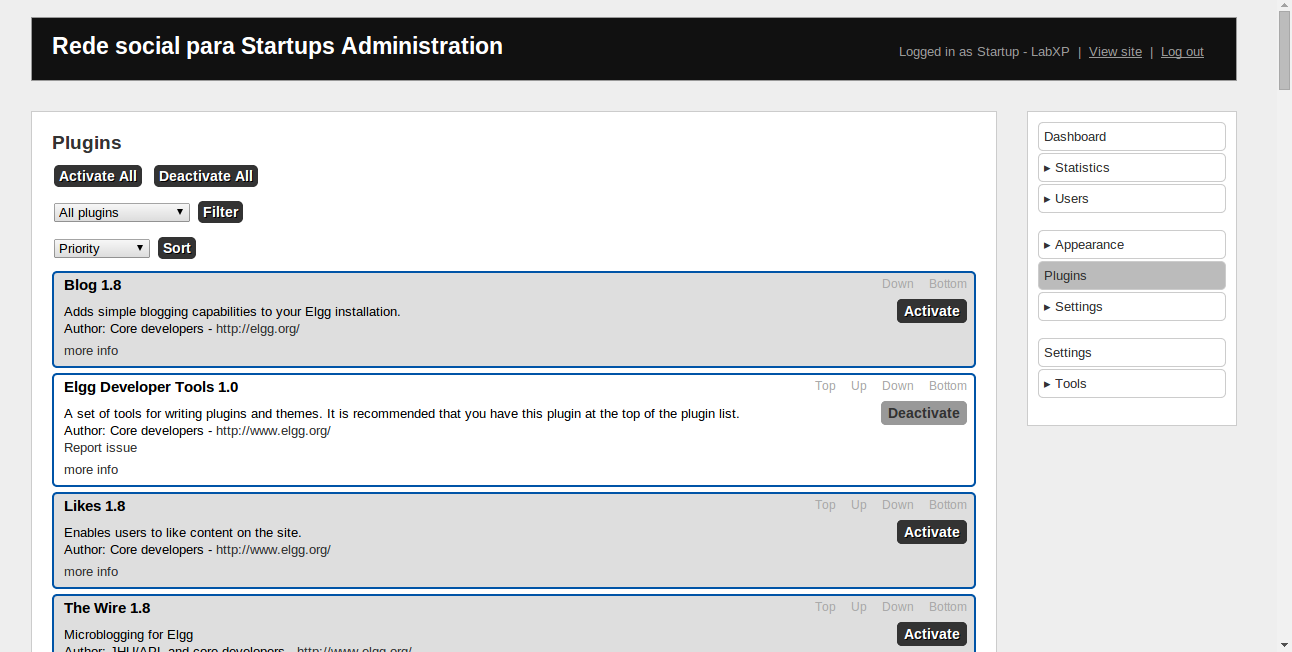
\includegraphics[scale=.35]{images/admin.png}
\caption{Janela de administrador da rede social}
\label{fig:admin}
\end{figure}


Para um melhor conhecimento do ELGG, sobre a pasta principal do projeto foi colocado um arquivo {\bf howto.txt}, onde se encontram alguns links e informação de tópicos de desenvolvimento e configuração da rede social desenvolvida.

\section{Monashees Plus Network}
A ideia principal da rede social interna na empresa Monashees Capital, é que os membros do portafólio de empresas e principais consultores (Venture Advisors) possam trocar perguntas, respostas ideias e experiencias para o agil desenvolvimento de todos os membros e startups que fazem parte da Monashees. \\

No primeiro protótipo da rede social se criaram e adaptaram vários plugins. Entre os principais Plugins desenvolvidos estão Filters, Home, People, e Venture Advisors.

\subsection{Plugin Filters}
O Plugin de Filter faz as principais operações de filtrado das diferentes entidades criadas por os outros plugins, o plugin Filter é usado para filtrar os usuários que fazem parte da rede social, para filtrar as perguntas ou entradas feitas por os usuários no plugin do Home, e para filtrar os Ventures Advisor criados pelo administrador do sistema. Veja a Figura \ref{fig:Home}.

\begin{figure}[htpb]
\centering
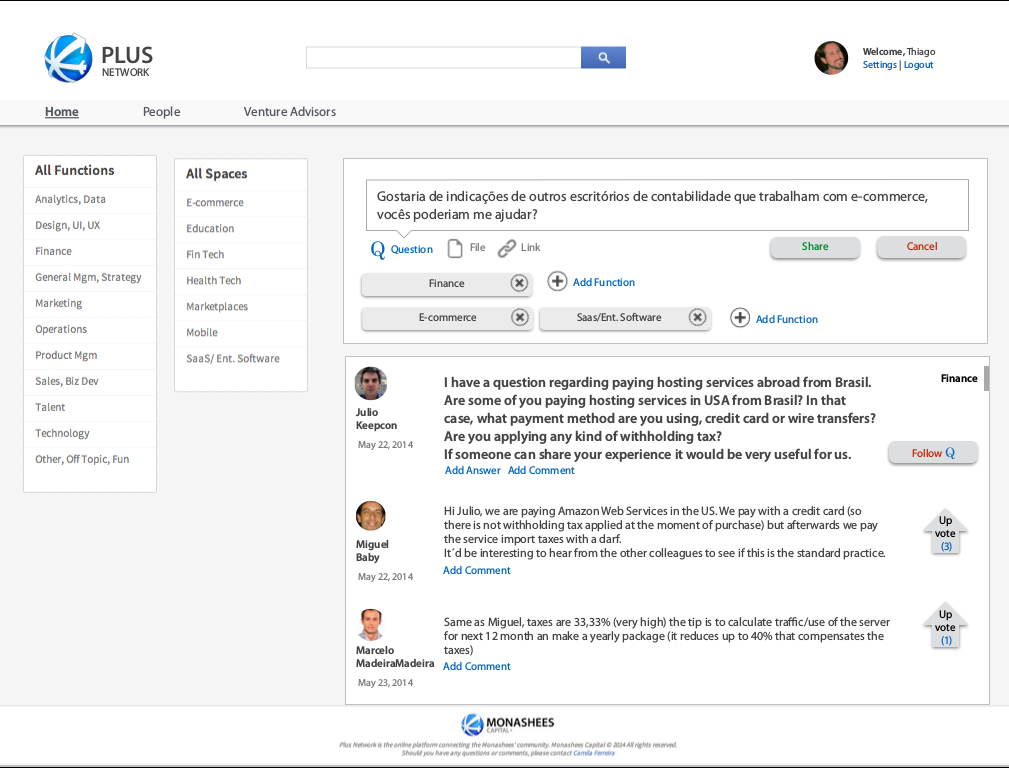
\includegraphics[scale=.35]{images/home.png}
\caption{Janela principal do plugin de Home}
\label{fig:Home}
\end{figure}

\subsection{Plugin Home}
No plugin de Home os usuários da rede social poderão submeter perguntas ou entradas ao sistemas filtrando elas por funções e espaços. Também o usuário poderá filtrar por funções e espaços as diferentes entradas que aprecem no painel principal de visualização Home.

\subsection{Plugin People}
Os usuários do sistema da rede social uma vez entram ao sistema por médio da rede social linkedin, terão que cadastrar as funções que ele faz no startup o empresa em que trabalham, estos dados são pedidos uma vez entram pelo linkedin e a janela de entrada é tal como se apresenta na Figura  \ref{fig:filters}. Esta informação é usada para a filtragem de usuários no plugin de People. 

\begin{figure}[htpb]
\centering
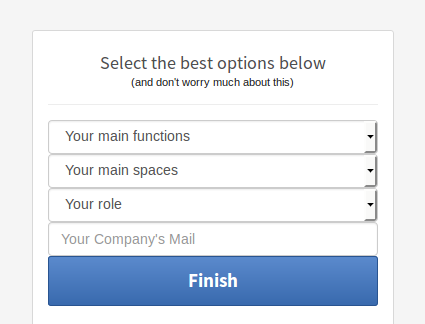
\includegraphics[scale=.5]{images/filters.png}
\caption{Janela de cadastro dos usuários da rede}
\label{fig:filters}
\end{figure}

\subsection{Plugin Ventures Advisor}
Os Ventures Advisor são colaboradores da Monashees, e eles brindam apoio às diferentes startups que fazem parte do porta-fólio de empresas e startups. O administrador do sistema cadastra e classifica os Ventures Advisors para que os usuários da rede social possam ter acesso à informação de contato destes consultores, veja a Figura \ref{fig:VA}.

\begin{figure}[htpb]
\centering
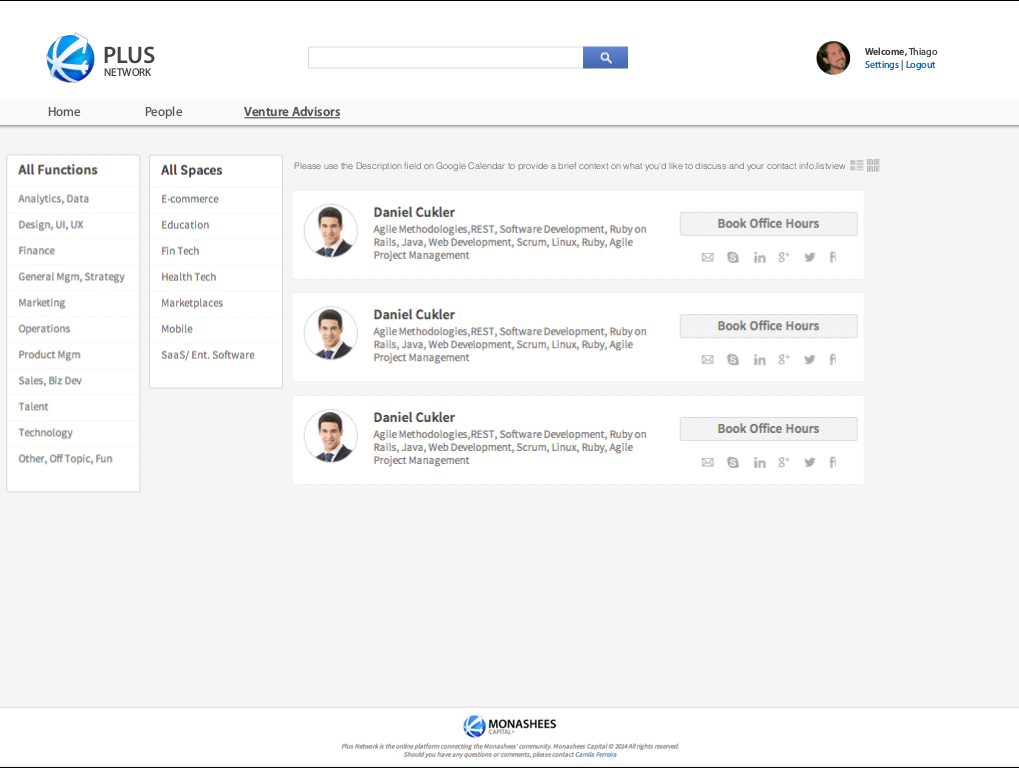
\includegraphics[scale=.325]{images/ventureAdvisor.png}
\caption{Janela de visualização de venture advisors para os usuários da rede social}
\label{fig:VA}
\end{figure}

\section{Testes}
O teste é muito importante no processo de desenvolvimento de um software, pois lhe garante mais qualidade, porém é uma atividade cara e demorada. Esta atividade pode inclusive consumir cerca de 50\% do total dos custos envolvidos no desenvolvimento de software. Dada a rapidez com que se queria a aplicação e o tempo gasto no aprendizagem da ferramenta foram criados testes automatizados de funcionalidades. A ferramenta para criar estes testes foi Selenium IDE\footnote{Selenium Projects - \url{http://docs.seleniumhq.org/download/http://docs.seleniumhq.org/download/}}, plugin do navegador Firefox Mozilla.

\subsection{Testes de Selenium}
Selenium IDE é um plugin do Firefox que grava e reproduz interações do usuário com o browser, veja Figura \ref{fig:Selenium}. No projeto baixado encontrará uma pasta {\texttt selenium-tests}, onde estão os arquivos de testes de funcionalidade que serão abertos com Selenium IDE.

\begin{figure}[htpb]
\centering
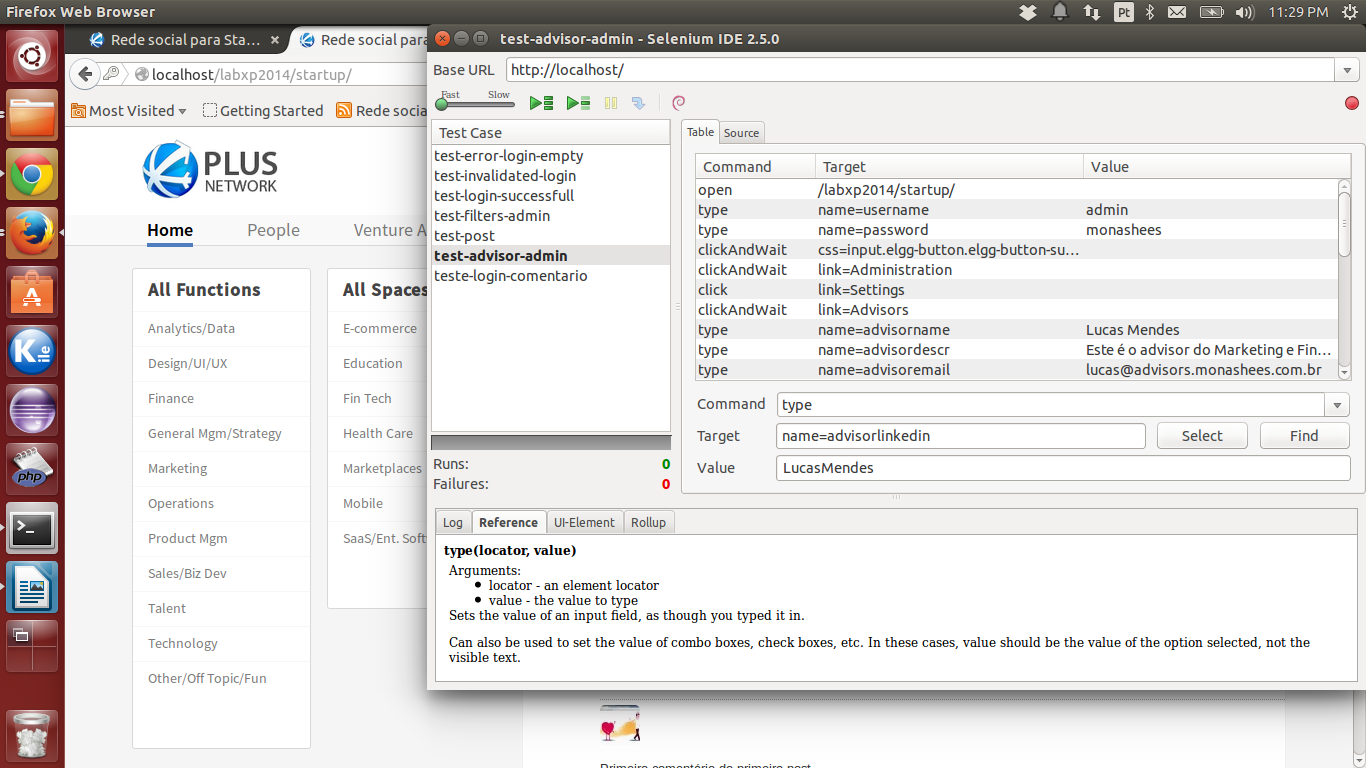
\includegraphics[scale=.325]{images/selenium.png}
\caption{Janela principal do Selenium IDE}
\label{fig:Selenium}
\end{figure}

\end{document}
